\section{光滑性}
\label{sec:smooth-lipschitz}

由第~\ref{chap:optimization}章的方向导数，当位移$\bm{p}$趋于零时，$f(\bm{x}+\bm{p})$与线性预测$f(\bm{x})+\langle\nabla f(\bm{x}),\bm{p}\rangle$的差比$\lVert\bm{p}\rVert_2$更快地趋于零。算法迈出的却是有限的一步。接下来要弄清：一次有限的移动之后，目标最多偏离线性预测多少？

\paragraph{贯穿本章的例子}
本章反复使用下面的二元二次目标：
\begin{equation}
 f(\bm{x})=\frac12\bigl(x_1^2+9x_2^2\bigr),\qquad \bm{x}^{(0)}=(9,1).
 \label{eq:smooth-running}
\end{equation}
它的Hessian是$\bm{H}=\operatorname{diag}(1,9)$，最优解是原点，$f^\star=0$。等高线是沿$x_1$方向拉长的椭圆，碗底像一条山谷。

在初始点算出目标值和梯度：
\[
 f(\bm{x}^{(0)})=45,\qquad \nabla f(\bm{x}^{(0)})=(9,9).
\]
这个例子所有的量都能手算，而两个方向的曲率相差$9$倍，足以暴露步长选择的主要现象。

\paragraph{梯度变化得多快}
线性预测把脚下的坡度当成一路不变。预测错多少，取决于走动时坡度变了多少。在例~\eqref{eq:smooth-running}中，两点的梯度之差是
\[
 \nabla f(\bm{u})-\nabla f(\bm{v})=\bm{H}(\bm{u}-\bm{v}).
\]
沿$x_1$方向移动单位长度，梯度改变$1$；沿$x_2$方向移动单位长度，梯度改变$9$。无论朝哪个方向走，单位位移引起的梯度变化都不超过$9$。

这个数就是坡度变化的限速。有了限速，站在一点上虽然看不见远处，却可以断定走出距离$r$之后坡度至多变化多少。对一般目标，我们要求这样的限速在关心的区域内统一存在。

\begin{definition}[梯度Lipschitz条件]
\label{def:smooth-lipschitz}
设$f:\mathbb{R}^n\to\mathbb{R}$可微，$\bm{U}\subseteq\mathbb{R}^n$，$L\geq0$。若对所有$\bm{u},\bm{v}\in\bm{U}$，
\begin{equation}
 \lVert\nabla f(\bm{u})-\nabla f(\bm{v})\rVert_2\leq L\lVert\bm{u}-\bm{v}\rVert_2,
 \label{eq:smooth-lipschitz}
\end{equation}
就说$\nabla f$在$\bm{U}$上满足\term{梯度Lipschitz条件}（gradient Lipschitz condition），也说$f$在$\bm{U}$上$L$光滑（$L$-smooth）。满足条件的$L$称为\term{光滑常数}（smoothness constant）。$\bm{U}=\mathbb{R}^n$时简称$f$是$L$光滑的。
\end{definition}

这个定义把第~\ref{chap:optimization}章只对二阶可微函数使用的$L$推广了：这里不要求Hessian存在。图~\ref{fig:smooth-gradient-cone}用一元函数的导数曲线说明条件的含义。以曲线上一点为顶点、作斜率为$\pm L$的两条直线，得到一个双锥形。条件~\eqref{eq:smooth-lipschitz}等于说，无论把顶点放在曲线的哪一点，整条曲线都留在锥内。

\begin{BookInlineFigure}
  \centering
  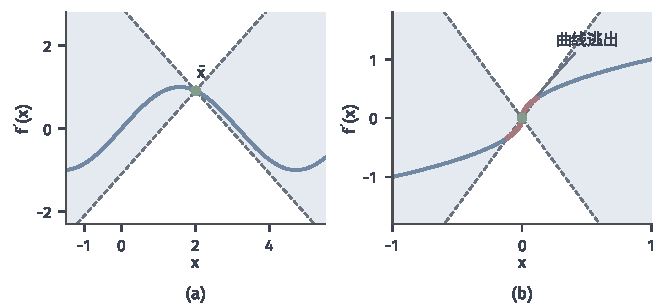
\includegraphics[width=112mm]{figures/05-optimization/02-smooth-optimization/matplotlib/smooth-gradient-cone/figure.pdf}
  \caption{梯度Lipschitz条件的几何含义。蓝线是导数曲线，浅蓝区域是从绿点出发、斜率为$\pm L$的双锥。(a)$f'(x)=\sin x$，取$L=1$，顶点放在$\bar{x}=2$，曲线留在锥内；顶点放在其他点时同样如此。(b)$f'(x)=\operatorname{sign}(x)\lvert x\rvert^{1/2}$，取$L=3$，顶点放在$0$，红色部分$\lvert x\rvert<1/9$逃出了锥；$L$再大，逃出的部分只是变短，永远存在。}
  \label{fig:smooth-gradient-cone}
\end{BookInlineFigure}

\paragraph{三个相近的条件}
“可微”“梯度连续”“梯度Lipschitz”是逐步加强的三个要求，图~\ref{fig:smooth-gradient-cone}(b)的函数正好落在中间。取$f(x)=\frac23\lvert x\rvert^{3/2}$，它处处可微，导数是
\[
 f'(x)=\operatorname{sign}(x)\lvert x\rvert^{1/2},
\]
这个导数也连续。但以$0$为参照点，
\[
 \frac{\lvert f'(x)-f'(0)\rvert}{\lvert x\rvert}=\lvert x\rvert^{-1/2},
\]
$x\to0$时趋于无穷，所以包含原点的任何区间上都没有光滑常数。

高阶可微也不能保证全局的常数。$f(x)=x^4$无穷次可微，而
\[
 \frac{\lvert f'(u)-f'(0)\rvert}{\lvert u\rvert}=4u^2,
\]
$u$变大时无界。限制在$[-R,R]$上时，$f''(x)=12x^2\leq12R^2$，常数$12R^2$随区域变大。所以说一个目标“光滑”时，要同时交代常数和它成立的区域。

\paragraph{下降引理}
有了坡度的限速，就能控制线性预测的误差。思路是把有限的位移分成无穷多小段累加：每一小段上的真实变化由该处的坡度决定，它与起点坡度之差不超过限速乘以已走的距离。

\begin{lemma}[下降引理]
\label{lem:smooth-descent}
设$f:\mathbb{R}^n\to\mathbb{R}$可微，并在集合$\bm{U}$上$L$光滑。若线段$\{\bm{x}+s\bm{p}:s\in[0,1]\}$落在$\bm{U}$中，则
\begin{equation}
 \bigl\lvert f(\bm{x}+\bm{p})-f(\bm{x})-\langle\nabla f(\bm{x}),\bm{p}\rangle\bigr\rvert
 \leq\frac{L}{2}\lVert\bm{p}\rVert_2^2.
 \label{eq:smooth-remainder}
\end{equation}
特别地，
\begin{equation}
 f(\bm{x}+\bm{p})\leq f(\bm{x})+\langle\nabla f(\bm{x}),\bm{p}\rangle+\frac{L}{2}\lVert\bm{p}\rVert_2^2.
 \label{eq:smooth-descent-lemma}
\end{equation}
\end{lemma}

\begin{proof}
令$\phi(s)=f(\bm{x}+s\bm{p})$，$s\in[0,1]$。由链式法则，
\[
 \phi'(s)=\langle\nabla f(\bm{x}+s\bm{p}),\bm{p}\rangle.
\]
线段在$\bm{U}$中，$\nabla f$沿线段Lipschitz，所以$\phi'$连续，微积分基本定理给出
\[
 f(\bm{x}+\bm{p})-f(\bm{x})=\int_0^1\langle\nabla f(\bm{x}+s\bm{p}),\bm{p}\rangle\,\mathrm{d}s.
\]

两边减去常数$\langle\nabla f(\bm{x}),\bm{p}\rangle$，并把它也写成$s$从$0$到$1$的积分，得到
\[
 f(\bm{x}+\bm{p})-f(\bm{x})-\langle\nabla f(\bm{x}),\bm{p}\rangle
 =\int_0^1\langle\nabla f(\bm{x}+s\bm{p})-\nabla f(\bm{x}),\bm{p}\rangle\,\mathrm{d}s.
\]

由Cauchy--Schwarz不等式和式~\eqref{eq:smooth-lipschitz}，被积函数的绝对值满足
\[
 \bigl\lvert\langle\nabla f(\bm{x}+s\bm{p})-\nabla f(\bm{x}),\bm{p}\rangle\bigr\rvert
 \leq Ls\lVert\bm{p}\rVert_2^2.
\]
对$s$从$0$积分到$1$，右端成为$\frac{L}{2}\lVert\bm{p}\rVert_2^2$，式~\eqref{eq:smooth-remainder}成立。去掉绝对值取上半部分，即得式~\eqref{eq:smooth-descent-lemma}。
\end{proof}

上界~\eqref{eq:smooth-descent-lemma}称为\term{下降引理}（descent lemma），它是后面证明目标下降的主要工具。把右端看成$\bm{p}$的函数，记作
\begin{equation}
 m_L(\bm{p})=f(\bm{x})+\langle\nabla f(\bm{x}),\bm{p}\rangle+\frac{L}{2}\lVert\bm{p}\rVert_2^2.
 \label{eq:smooth-upper-model}
\end{equation}
这是一个在当前点与$f$相切、开口向上的二次函数，像一只倒扣过来的碗从上方盖住了$f$。下半部分则是开口向下的二次函数，从下方托住$f$。

图~\ref{fig:smooth-upper-lower-model}画出$f(x)=1-\cos x$的情形。这里$f''(x)=\cos x$，取值在$[-1,1]$内，$L=1$，当前点$x^{(0)}=2$。整条曲线都夹在两条抛物线之间。

\begin{BookInlineFigure}
  \centering
  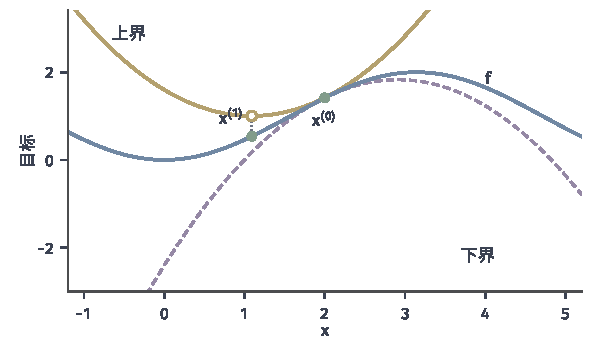
\includegraphics[width=100mm]{figures/05-optimization/02-smooth-optimization/matplotlib/smooth-upper-lower-model/figure.pdf}
  \caption{$f(x)=1-\cos x$在$x^{(0)}=2$处的二次上界（黄线）与二次下界（紫色虚线），$L=1$。空心点是上界的最低点，其正下方的绿点$x^{(1)}=2-\sin2$是目标在同一位置的真实值，后者不高于前者。}
  \label{fig:smooth-upper-lower-model}
\end{BookInlineFigure}

\paragraph{上界怎样限制一步更新}
上界的用途在于，它把“走到哪里”变成一个能解的问题。式~\eqref{eq:smooth-upper-model}对$\bm{p}$求梯度并令其为零，最低点是
\[
 \bm{p}=-\frac{1}{L}\nabla f(\bm{x}).
\]

代回式~\eqref{eq:smooth-descent-lemma}，得到一步能够保证的下降量：
\begin{equation}
 f\Bigl(\bm{x}-\frac{1}{L}\nabla f(\bm{x})\Bigr)\leq f(\bm{x})-\frac{1}{2L}\lVert\nabla f(\bm{x})\rVert_2^2.
 \label{eq:smooth-model-min}
\end{equation}

这个结论的意思是：只要落点在碗的最低处，真实目标不会比碗底更高。在图~\ref{fig:smooth-upper-lower-model}的例子里，$\sin2\approx0.909$，当前值、碗底值和真实落点值分别是
\[
 f(2)\approx1.416,\qquad m_L(-0.909)\approx1.003,\qquad f(1.091)\approx0.538.
\]
保证的下降量是$0.413$，实际下降$0.878$。上界不紧，但它不需要试探就能给出保证。

回到例~\eqref{eq:smooth-running}。此时$L=9$，当前点的上界最低点是$\bm{x}^{(1)}=(9,1)-\frac19(9,9)=(8,0)$，碗底高度与真实值分别是
\[
 f(\bm{x}^{(0)})-\frac{\lVert\bm{g}^{(0)}\rVert_2^2}{2L}=45-9=36,\qquad f(\bm{x}^{(1)})=32.
\]
图~\ref{fig:smooth-isotropic-model}显示了这一步的几何。上界的等高线是圆，真实目标的等高线是椭圆。经过当前点的圆完全落在经过当前点的椭圆之内，所以圆内每一点都比当前点低。

\begin{BookInlineFigure}
  \centering
  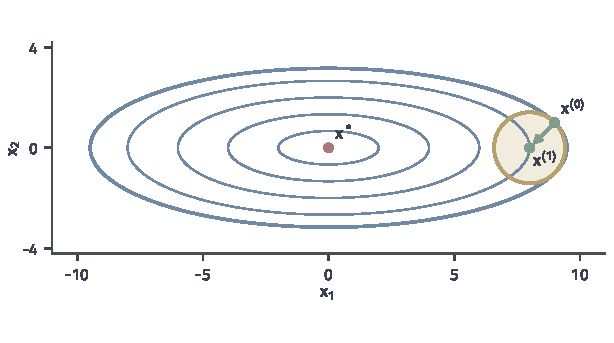
\includegraphics[width=104mm]{figures/05-optimization/02-smooth-optimization/matplotlib/smooth-isotropic-model/figure.pdf}
  \caption{各向同性的上界盖住各向异性的目标。蓝线是例~\eqref{eq:smooth-running}的等高线，粗线经过$\bm{x}^{(0)}$。黄圆是上界$m_L$经过$\bm{x}^{(0)}$的等高线，圆心$\bm{x}^{(1)}=(8,0)$是上界的最低点，绿色箭头是步$-\bm{g}^{(0)}/L$。圆的半径是$\lVert\bm{g}^{(0)}\rVert_2/L=\sqrt2$，比到最优解的距离小得多。}
  \label{fig:smooth-isotropic-model}
\end{BookInlineFigure}

这个图也说明了上界的弱点。它只知道一个数$L$，必须按最陡的方向处处提防，所以朝平坦的$x_1$方向也不敢多走。碗的类比到这里就要打折扣：真实地形是一条长谷，而这只碗是圆的，它保证安全，却不描述谷的走向。

\paragraph{局部模型能信多远}
下降引理有一句前提：线段要落在$L$成立的区域内。这句话不能省。取$f(x)=x^4$，当前点$x^{(0)}=1$，导数是$4$。在$[-1,1]$上$f''\leq12$，取$L=12$，上界是
\[
 m(x)=1+4(x-1)+6(x-1)^2.
\]

上界与目标之差可以因式分解，
\[
 f(x)-m(x)=(x-1)^3(x+3).
\]
当$-3\leq x\leq1$时它不大于零，上界盖得住；当$x>1$或$x<-3$时它大于零，上界失效。

图~\ref{fig:smooth-model-range}(b)放大了当前点附近：只要向右走一点点，$f''$就超过$12$，上界立刻盖不住。向左，上界一直盖到$x=-3$，比$L$成立的区间$[-1,1]$更远，因为靠近当前点那段曲率小于$12$，积累的余量抵消了后来过大的曲率。引理只承诺线段在区域内时成立，区域外可能成立，也可能不成立。

\begin{BookInlineFigure}
  \centering
  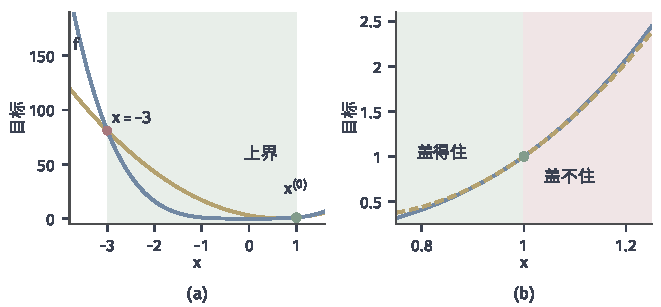
\includegraphics[width=112mm]{figures/05-optimization/02-smooth-optimization/matplotlib/smooth-model-range/figure.pdf}
  \caption{局部常数的有效范围。$f(x)=x^4$（蓝线），在$x^{(0)}=1$处用$[-1,1]$上的常数$L=12$作上界（黄线）。(a)浅绿区域$[-3,1]$内上界盖住目标，$x=-3$是另一个交点。(b)放大当前点附近：左侧盖得住；右侧浅红区域$f''>12$，上界立刻盖不住，虚线低于蓝线。}
  \label{fig:smooth-model-range}
\end{BookInlineFigure}

\paragraph{上界与凸性无关}
上界$m_L$永远是凸函数，这容易让人以为$L$光滑带有某种凸性。其实两件事互不蕴含。$L$限制的是弯曲的绝对大小，凸性限制的是弯曲的方向。表~\ref{tab:smooth-vs-convex}用四个一元函数列出全部组合。

\begin{BookInlineTable}
  \centering
  \begin{tabular}{@{}lll@{}}
    \toprule
     & 凸 & 非凸\\
    \midrule
    全局$L$光滑 & $x^2/2$，$L=1$ & $1-\cos x$，$L=1$\\
    无全局常数 & $x^4$ & $x^4-x^2$\\
    \bottomrule
  \end{tabular}
  \caption{全局光滑性与凸性互不蕴含。第一行的函数二阶导数有界，第二行无界；第一列的函数二阶导数非负，第二列会取负值。}
  \label{tab:smooth-vs-convex}
\end{BookInlineTable}

两者对局部模型的贡献也不同。光滑性给出二次上界，告诉我们一步最多变差多少，由此保证下降。凸性把式~\eqref{eq:smooth-remainder}的下半部分从开口向下的抛物线提高到切平面，也就是第~\ref{chap:optimization}章的支撑不等式，由此才能从一点的信息推断全局。$1-\cos x$在$x^{(0)}=3$附近上界依然成立，但这里的小梯度不说明接近最小点。

\paragraph{下水平集上的常数}
实际目标常常没有全局的$L$，例如$x^4$。好在下降算法不必到处走：只要每步都不升高，迭代点就留在初始的下水平集里。下面的引理说明，$L$只在下水平集上成立时，只要步长受限，这一步的整条线段就不会走出去，下降引理可以照用。

\begin{lemma}[梯度步留在下水平集内]
\label{lem:smooth-sublevel}
设$f:\mathbb{R}^n\to\mathbb{R}$可微，$\bm{S}=\{\bm{z}:f(\bm{z})\leq a\}$，$f$在$\bm{S}$上$L$光滑，$L>0$。设$\bm{x}\in\bm{S}$，$\bm{g}=\nabla f(\bm{x})\neq\bm{0}$，$0<\alpha<2/L$。则线段$\{\bm{x}-s\bm{g}:s\in[0,\alpha]\}$落在$\bm{S}$内，并且
\begin{equation}
 f(\bm{x}-\alpha\bm{g})\leq f(\bm{x})-\alpha\Bigl(1-\frac{L\alpha}{2}\Bigr)\lVert\bm{g}\rVert_2^2.
 \label{eq:smooth-sublevel-step}
\end{equation}
\end{lemma}

\begin{proof}
令$\phi(s)=f(\bm{x}-s\bm{g})$。设$\bar{s}$是使$\phi$在$[0,\bar{s}]$上始终不超过$a$的最大的$\bar{s}\in[0,\alpha]$，由连续性，这个最大值取得到。因为$\phi'(0)=-\lVert\bm{g}\rVert_2^2<0$且$\phi(0)\leq a$，所以$\bar{s}>0$。

线段$\{\bm{x}-s\bm{g}:s\in[0,\bar{s}]\}$在$\bm{S}$中，对$\bm{p}=-\bar{s}\bm{g}$用下降引理，得到
\[
 \phi(\bar{s})\leq f(\bm{x})-\bar{s}\Bigl(1-\frac{L\bar{s}}{2}\Bigr)\lVert\bm{g}\rVert_2^2<f(\bm{x})\leq a.
\]
严格不等式成立，是因为$0<\bar{s}<2/L$。

若$\bar{s}<\alpha$，由$\phi(\bar{s})<a$和连续性，$\phi$在$\bar{s}$右侧一小段上仍不超过$a$，与$\bar{s}$的取法矛盾。所以$\bar{s}=\alpha$，上面的不等式就是式~\eqref{eq:smooth-sublevel-step}。
\end{proof}

用$f(x)=x^4$、$x^{(0)}=1$核对一下。取$a=1$，$\bm{S}=[-1,1]$，$L=12$，于是$\alpha<1/6$时引理适用。取$\alpha=1/12$，走到$x=2/3$，式~\eqref{eq:smooth-sublevel-step}给出的上界和真实值分别是
\[
 1-\frac{1}{12}\cdot\frac12\cdot16=\frac13,\qquad f\Bigl(\frac23\Bigr)=\frac{16}{81}\approx0.198.
\]
若取$\alpha=1/2$，超出了范围，迭代在$1$和$-1$之间来回跳，目标不再下降。

\paragraph{目标差控制梯度}
式~\eqref{eq:smooth-model-min}还有一个推论。设$f$在$\mathbb{R}^n$上$L$光滑，并且下有界，记$f_{\inf}=\inf f$。式~\eqref{eq:smooth-model-min}的左端不低于$f_{\inf}$，移项得到
\begin{equation}
 \frac{1}{2L}\lVert\nabla f(\bm{x})\rVert_2^2\leq f(\bm{x})-f_{\inf}.
 \label{eq:smooth-gap-gradient}
\end{equation}
第~\ref{chap:optimization}章在强凸的条件下证过同样的不等式，这里既不要求凸，也不要求二阶可微，甚至不要求最优解存在。直观上，若坡度很陡而离下界很近，沿坡度走一步就会跌破下界。

\paragraph{用Hessian估计光滑常数}
定义~\ref{def:smooth-lipschitz}要比较所有点对，直接检验并不方便。目标二阶可微时，梯度的变化率就是Hessian，常数可以从Hessian读出。

\begin{theorem}[Hessian与光滑常数]
\label{thm:smooth-hessian}
设$\bm{U}\subseteq\mathbb{R}^n$是凸开集，$f$在$\bm{U}$上二阶连续可微。则$f$在$\bm{U}$上$L$光滑，当且仅当对所有$\bm{z}\in\bm{U}$，
\begin{equation}
 \lVert\nabla^2f(\bm{z})\rVert_2\leq L.
 \label{eq:smooth-hessian-bound}
\end{equation}
\end{theorem}

\begin{proof}
先设式~\eqref{eq:smooth-hessian-bound}成立。对$\bm{u},\bm{v}\in\bm{U}$，线段留在$\bm{U}$中，这里用到了$\bm{U}$的凸性。沿线段对梯度积分，得到
\[
 \nabla f(\bm{u})-\nabla f(\bm{v})=\int_0^1\nabla^2f\bigl(\bm{v}+s(\bm{u}-\bm{v})\bigr)(\bm{u}-\bm{v})\,\mathrm{d}s.
\]
取范数，积分的范数不超过范数的积分，被积向量的范数不超过$L\lVert\bm{u}-\bm{v}\rVert_2$，即得式~\eqref{eq:smooth-lipschitz}。

反过来，设$f$在$\bm{U}$上$L$光滑。取$\bm{z}\in\bm{U}$和单位向量$\bm{v}$，$s>0$充分小时$\bm{z}+s\bm{v}\in\bm{U}$，于是
\[
 \Bigl\lVert\frac{\nabla f(\bm{z}+s\bm{v})-\nabla f(\bm{z})}{s}\Bigr\rVert_2\leq L.
\]
令$s\downarrow0$，左端趋于$\lVert\nabla^2f(\bm{z})\bm{v}\rVert_2$。对所有单位向量取上确界，即得式~\eqref{eq:smooth-hessian-bound}。
\end{proof}

定理说明，最小的光滑常数恰好是$\bm{U}$上$\lVert\nabla^2f\rVert_2$的上确界。对称矩阵的谱范数等于特征值绝对值的最大者，定义与性质可参考\BookChapterRef{chap:eigen-spectral-decomposition}{卷二第6章“谱分解”}。要注意绝对值：负曲率同样计入$L$，例如$\frac12(x_1^2-4x_2^2)$的$L=4$。

几个常见情形可以直接写出。二次目标$\frac12\bm{x}^\top\bm{H}\bm{x}$的$L=\max_i\lvert\lambda_i(\bm{H})\rvert$，例~\eqref{eq:smooth-running}中$L=9$。最小二乘$\frac12\lVert\bm{A}\bm{x}-\bm{b}\rVert_2^2$的Hessian是$\bm{A}^\top\bm{A}$，所以$L=\lVert\bm{A}\rVert_2^2$。第~\ref{chap:optimization}章的二次拟合实例，Hessian的特征值是$2+\gamma$和$\gamma$，所以$L=2+\gamma$。

非二次目标要在整个区域上取上确界。考虑
\[
 f(\bm{x})=\cos(x_1+x_2)+\frac12\lVert\bm{x}\rVert_2^2,
\]
记$c=\cos(x_1+x_2)$，Hessian是
\[
 \nabla^2f(\bm{x})=\bm{I}-c\begin{bmatrix}1&1\\1&1\end{bmatrix}.
\]
方向$(1,-1)$上的特征值是$1$，方向$(1,1)$上的特征值是$1-2c$。$c$取遍$[-1,1]$时，$1-2c$取遍$[-1,3]$，所以$L=3$。这个目标在$c>1/2$的区域非凸，却是全局$3$光滑的。

\paragraph{矩阵太大时怎样估计}
维数很大时，特征值不便精确算出。有两类办法，它们的方向相反。第一类给上界，只用矩阵的元素：对称矩阵$\bm{H}$的谱范数不超过最大的绝对行和$\lVert\bm{H}\rVert_\infty$，也不超过Frobenius范数$\lVert\bm{H}\rVert_{\mathrm{F}}$；半正定时还不超过迹。第二类给下界：从向量$\bm{v}$出发反复乘$\bm{H}$，这个做法称为幂迭代，再计算Rayleigh商$\bm{v}^\top\bm{H}\bm{v}/\bm{v}^\top\bm{v}$。它不需要写出矩阵，只要能算矩阵向量积。

下面的矩阵用来比较这两类估计：
\[
 \bm{H}=\begin{bmatrix}2&1&0\\1&3&1\\0&1&2\end{bmatrix}.
\]
它的特征值是$1,2,4$，所以$L=4$。三个上界分别是
\[
 \lVert\bm{H}\rVert_\infty=5,\qquad \lVert\bm{H}\rVert_{\mathrm{F}}=\sqrt{21}\approx4.58,\qquad \operatorname{tr}\bm{H}=7.
\]

幂迭代从$\bm{v}=(1,1,1)$出发，前三次的Rayleigh商是
\[
 \frac{11}{3}\approx3.667,\qquad \frac{171}{43}\approx3.977,\qquad \frac{2731}{683}\approx3.999.
\]
图~\ref{fig:smooth-hessian-estimates}把两类估计放在一起。上界偏保守，用它得到的步长偏小，但步长是安全的。幂迭代逼近得快，却总从下方接近真值，直接拿来算步长可能略微超出安全范围。实践中常把幂迭代的结果乘一个略大于$1$的系数。

\begin{BookInlineFigure}
  \centering
  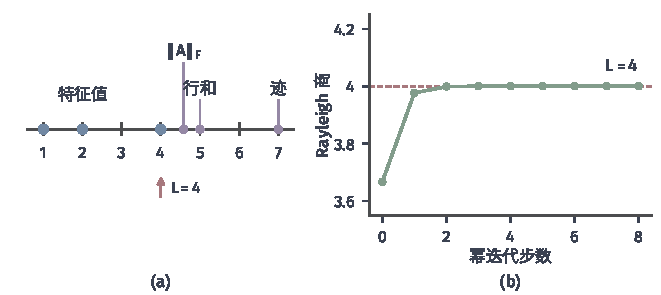
\includegraphics[width=112mm]{figures/05-optimization/02-smooth-optimization/matplotlib/smooth-hessian-estimates/figure.pdf}
  \caption{估计$L$的两类办法，矩阵见正文，特征值为$1,2,4$。(a)数轴上的蓝点是特征值，紫点是由元素算出的三个上界：Frobenius范数约$4.58$、最大绝对行和$5$、迹$7$，它们都不低于$L=4$。(b)幂迭代的Rayleigh商随步数增加，始终不超过$L$（红色虚线）。}
  \label{fig:smooth-hessian-estimates}
\end{BookInlineFigure}

对非二次目标，还要处理$\bm{z}$变化带来的麻烦：在一点上的估计并不代表整个区域。下一节的回溯线搜索正是为不知道$L$的情形准备的，它把估计常数换成了用真实函数值检验。
